%%%%%%%%%%%%%%%%%%%%%%%%%%%%%%%%%%%%%%%%%%%%%%%%%%%%%%%%%%%%%%%%%%
%%%%%%%% ICML 2014 EXAMPLE LATEX SUBMISSION FILE %%%%%%%%%%%%%%%%%
%%%%%%%%%%%%%%%%%%%%%%%%%%%%%%%%%%%%%%%%%%%%%%%%%%%%%%%%%%%%%%%%%%

% Use the following line _only_ if you're still using LaTeX 2.09.
%\documentstyle[icml2014,epsf,natbib]{article}
% If you rely on Latex2e packages, like most moden people use this:
\documentclass{article}

% use Times
\usepackage{times}
% For figures
\usepackage{xcolor}
\usepackage{graphicx} % more modern
%\usepackage{epsfig} % less modern
\usepackage{subfigure} 

% For citations
\usepackage{natbib}

% For algorithms
\usepackage{algorithm}
\usepackage{algorithmic}

\usepackage{amsmath}
\usepackage{amssymb}
\usepackage{amsthm}

% As of 2011, we use the hyperref package to produce hyperlinks in the
% resulting PDF.  If this breaks your system, please commend out the
% following usepackage line and replace \usepackage{icml2014} with
% \usepackage[nohyperref]{icml2014} above.
\usepackage{hyperref}

% Packages hyperref and algorithmic misbehave sometimes.  We can fix
% this with the following command.
\newcommand{\theHalgorithm}{\arabic{algorithm}}

\newcommand{\YFcomment}[1]{\marginpar{\footnotesize{{\bf YF:} #1}}}
\newcommand{\SCcomment}[1]{\marginpar{\footnotesize{{\bf SC:} #1}}}

\newtheorem{theorem}{Theorem}
\newtheorem{lemma}[theorem]{Lemma}
\newtheorem{collorary}[theorem]{Collorary}

% Employ the following version of the ``usepackage'' statement for
% submitting the draft version of the paper for review.  This will set
% the note in the first column to ``Under review.  Do not distribute.''
\usepackage{icml2014} 
% Employ this version of the ``usepackage'' statement after the paper has
% been accepted, when creating the final version.  This will set the
% note in the first column to ``Proceedings of the...''
%\usepackage[accepted]{icml2014}


% The \icmltitle you define below is probably too long as a header.
% Therefore, a short form for the running title is supplied here:
\icmltitlerunning{CHANGE ME}

\begin{document} 

\twocolumn[
\icmltitle{TBD}

% It is OKAY to include author information, even for blind
% submissions: the style file will automatically remove it for you
% unless you've provided the [accepted] option to the icml2014
% package.
\icmlauthor{Sunsern Cheamanunkul}{scheaman@eng.ucsd.edu}
\icmladdress{UCSD,
            9500 Gilman Dr., La Jolla, CA 92093}
\icmlauthor{Yoav Freund}{yfreund@eng.ucsd.edu}
\icmladdress{UCSD,
            9500 Gilman Dr., La Jolla, CA 92093}

% You may provide any keywords that you 
% find helpful for describing your paper; these are used to populate 
% the "keywords" metadata in the PDF but will not be shown in the document
\icmlkeywords{boring formatting information, machine learning, ICML}

\vskip 0.3in
]

\begin{abstract} 
TODO
\end{abstract} 

\section{Introduction}
\label{sec:intro}

We consider the $k$-nearest neighbor ($k$-NN) classification rule for
multiclass classification problems where the number of classes $m >
2$. Given a set of training examples, the $k$-NN rule predicts the
label of a new example with the majority of the class labels among its
$k$ nearest neighbors. Fix and Hodges~\cite{Fix1951} show that,
asymptotically, the $k$-NN rule achieves the Bayes error rate $r^*$ by
choosing a large enough $k$ but small compared to the number of
examples $n$. Nonetheless, when $n$ is small, there is no guarantee of
how well the $k$-NN algorithm will perform. 

Additionaly, Cover and Hart~\cite{Cover1967} show that, when $k = 1$,
the aymptotic error rate of the $1$-NN rule is upperbounded by $r^*(2
- \frac{m}{m-1}r^*)$. This result suggests that at least a half of the
class information is contained in the nearest neighbor. When the
nearest neighbor does not have all of the class information, it is
possible that the missing class information could be extracted from
other examples in the neighborhood.

In this paper, we propose a modification to the $k$-NN rule which
potentially leverages additional information from the non-majority
class labels in the neighborhood to improve the classification
accuracy. Our approach makes a prediction based on the entire
distribution of the class labels in the neighborhood instead of just
the majority. While the majority rule works well in most cases, it
completely ignores the information from the minority classes which, in
some cases, can contain crucial information.

To motivate our approach, consider the following example. Suppose
there are 3 classes of examples where each class is generated
according to each of the one-dimensional normal distributions depicted in
Figure~\ref{fig:toy_example}. Even though the example $x$ in
Figure~\ref{fig:toy_example} is of class A but it is likely that the
majority of class labels in the neighborhood of $x$ is class B. In
such case, the majority rule will predict class B. However, if we
consider the rest of the examples in the neighborhood of $x$ and we
rarely observe examples from class C, then a better prediction would
have been class A.

\begin{figure}[ht]
\vskip 0.2in
\begin{center}
\centerline{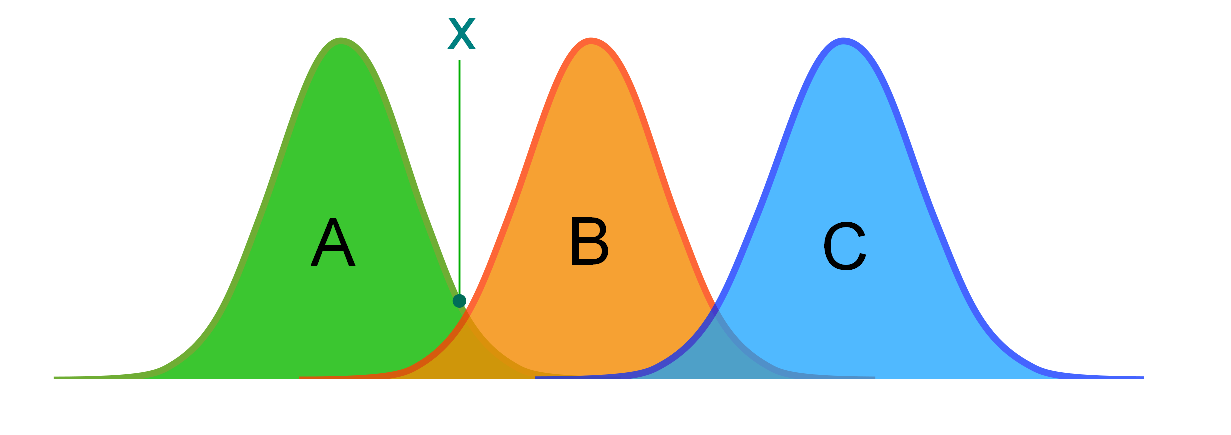
\includegraphics[width=\columnwidth]{figures/toy_example.eps}}
\caption{A toy example showing that the majarity rule (ignoring
  information about class C in the neighborhood) can be
  sub-optimal. Based on the majority rule, the example $x$ of class A
  can be misclassified as class B. However, the rare occurences of
  examples of class C in the neighborhood of $x$ can provide
  useful information regarding the true label of $x$.}
\label{fig:toy_example}
\end{center}
\vskip -0.2in
\end{figure} 

Our approach is related to work on learning label embeddings~
\cite{Collins2009, Bengio2010}. The main difference is that our approach is far
simpler, does not require any convex optimizations and can be
seemlessly integrated into the $k$-NN framework. Another related work
is \cite{Bilmes2001} which introduces a bias term to the likelihood ratio
testing which is justified by the difference between the estimated and
the true class conditional probability.

This paper is organized as follows. In Section~\ref{sec:background},
we describe the framework and the notations. In
Section~\ref{sec:min_kl}, we describe our approach and
justification. In Section~\ref{sec:results}, we present experiments
comparing our approach with the traditional $k$-NN algorithm using
both synthetic data and real-world data. Then, we discuss the results
in Section~\ref{sec:discussion} and conclude the paper in
Section~\ref{sec:conclusion}.

\section{Background}
\label{sec:background}

\newcommand{\X}{\mathcal{X}}
\newcommand{\Y}{\mathcal{Y}}
\newcommand{\trainset}{\mathcal{S}}

Let $\trainset = \{ (x_1,y_1,) \ldots (x_n,y_n)\}$ be a set of
training examples where each instance $x_i$ comes from an example
space $\X$ of which the distance between any two examples is measured by
$d(\cdot,\cdot)$. Without loss of generality, we assume that each
label $y_i$ takes on a value from $\Y = \{1,2,\ldots,m\}$.

\newcommand{\nh}{\mathcal{N}}
\newcommand{\Pemp}{\widehat{\mathbf{P}}_{(x,n,k)}}
\newcommand{\Ptrue}{\mathbf{P}_{(x)}}

Let $\nh_k(x)$ denote the neighborhood of size $k$ of an example $x
\in \X$ with respect to the distance measure $d$. The traditional
$k$-NN rule predicts the label of an example $x$ with the majority of
the labels in $\nh_k(x)$. More formally, given $x$ and $\nh_k(x)$, we
can define an empirical distribution $\Pemp$ such that, for each $i \in \Y$, 
\[
\Pemp(i) = \frac{\#\{ \mbox{occurrences of label } i \mbox{ in } \nh_k(x)\}}{k}
\]
The $k$-NN rule predicts the label $\hat{y}$ such that
\[
\hat{y} = \arg\max_{i \in \Y} \: \Pemp(i)
\]

For any example $x \in \X$, we can consider the true class
distribution of $x$, $\Ptrue$ which is given by, for each $i \in \Y$,
\[
\Ptrue(i) = \Pr(Y=i | X=x)
\]
Under certain assumptions, it is shown in \cite{Fix1951} that,
for every class label $i \in \Y$, 
\[
\lim_{\substack{n \to \infty\\k \to \infty\\k/n \to 0}} \Pemp(i) = \Ptrue(i)
\]
Therefore, the majority rule is asymptotically optimal. However, in
the finite sample case, it can be sub-optimal due to the discrepancy
between the empirical distribution $\Pemp$ and the true distribution
$\Ptrue$ as demonstrated by the toy example in
Figure~\ref{fig:toy_example}.

\section{Minimizing KL-Divergence Approach}

\newcommand{\dkl}{D_{\mathrm{KL}}}
\newcommand{\Qemp}{\widehat{\mathbf{Q}}_(j,n,k)}
\newcommand{\Qtrue}{\mathbf{Q}_(j)}

%%%%%%%%%%%
\iffalse
\fi
%%%%%%%%%%%

We propose a modification to the $k$-NN rule that predicts the class
label based on the entire class distribution $\Pemp$ instead of just
the mode of $\Pemp$. Given a training set $\trainset$ of size $n$ and
the neighborhood of size $k$, we define, for each class $j$, an
empirical center distribution $\Qemp$ as
\[
\Qemp(i) = \frac{\sum_{(x,j) \in \trainset_j} \Pemp(i)}{|\trainset_j|}
\]
where $\trainset_j = \{ (x,y) \in S | y = j \}$.  To classify a new
example $x$, the empirical class distribution $\Pemp$ is compared to
each of the center distributions $\Qemp$ with respect to some distance
measure $g(\cdot ; \cdot)$ and the class label that minimizes the
distance is then predicted. More formally, the predicted label
$\hat{y}$ is given by
\[
\hat{y} = \arg\min_{j \in \Y} \: g(\Pemp ; \Qemp)
\]

Technically, the choice of the function $g$ depends on the data but,
in this paper, we will give a justification for when $g$ is the
KL-divergence. The KL-divergence $\dkl$ between two
distributions $\mathbf{P}$ and $\mathbf{Q}$ is defined by
\[
\dkl(\mathbf{P} || \mathbf{Q}) = \sum_i \mathbf{P}(i) \log \frac{\mathbf{P}(i)}{\mathbf{Q}(i)}
\]

\newcommand{\Pexpected}{\tilde{\mathbf{P}}^{(x,n,k)}}

Next, we will give a justification for our approach for finite $n$ and
$k$. Let $\Qtrue$ denote the true center distribution for class $j$
which is given by
\[
\Qtrue = \int_x \Ptrue(j) \Ptrue
\]
For finite $n$ and $k$, we define the expected class distribution $\Pexpected$ for an example
$x$ as
\[
\Pexpected = \mathbf{E}[\Pemp]
\]








We show that, when the true class distribution $\Ptrue$ for each
example $x$ of class $j$ in the training set $\trainset$ is identical
to $\Qemp$, the KL-divergence is optimal. The proof is
given by Lemma~\ref{lemma:dkl} and Collorary~\ref{col:min_dkl}. 

\newcommand{\sampleYK}{y^k}
\newcommand{\sampleEmpDist}{\mathbf{P}_{y^k}}
\newcommand{\Q}{\mathbf{Q}}

Let $\sampleYK = [y_1, \ldots, y_k]$ denote a sample of size $k$ drawn IID
from a fixed distribution over $Y$ and let $\sampleEmpDist$ denote the
empirical distribution induced by the sample
$\sampleYK$. Specifically,
\[
\sampleEmpDist(i) = \frac{\#\{ \mbox{occurrences of } i \mbox{ in } y^k\}}{k}
\]

\begin{lemma}
\label{lemma:dkl}
For any distribution $\Q$ and for any sample $\sampleYK$ (not neccessarily
drawn from $\Q$), the likelihood of $\sampleYK$ drawn from $\Q$ is given by
\[
\Q(y^k) = 2^{-k(H(\sampleEmpDist) + \dkl\sampleEmpDist || \Q))}
\]
\end{lemma}
\begin{proof}
  \begin{align*}
    \Q(y^k) 
&= \prod_{l=1}^k \Q(y_l)\\ 
&= \prod_{j \in \Y} Q(j)^{n\sampleEmpDist(j)}\\ 
&= \prod_{j \in \Y} 2^{n\sampleEmpDist(j) \log \Q(j)}\\ 
&= \prod_{j \in \Y} 2^{n(\sampleEmpDist(j) \log \Q(j) - \sampleEmpDist(j) \log \sampleEmpDist(j) + \sampleEmpDist(j) \log \sampleEmpDist(j))}\\ 
&= 2^{k \sum_{j \in \Y} (-\sampleEmpDist(j) \log \frac{\sampleEmpDist(j)}{\Q(j)} + \sampleEmpDist(j) \log \sampleEmpDist(j))}\\ 
&= 2^{k(-\dkl(\sampleEmpDist||\Q) - H(\sampleEmpDist))}\\
  \end{align*}
\end{proof}

\begin{collorary}
\label{col:min_dkl}
Given a set of distributions $\mathcal{Q} = \{\Q_1,\Q_2, \ldots,
\Q_{m}\}$ and a sample $\sampleYK$ drawn from any distribution, the
likelihood of $\sampleYK$ is maximized under $\Q_{i^*}$ if and only if
the KL-divergence from $\sampleEmpDist$ to $\Q_{i^*}$ is minimized.
\[
 i^* = \arg\max_{i \in \Y} \log \Q_i(y^k) = \arg\min_{i \in \Y} \dkl(\sampleEmpDist||\Q_i)
\]
\end{collorary}
\begin{proof}
  Applying Lemma~\ref{lemma:dkl}, we have
  \begin{align*}
    \Q_i(y^k) &= 2^{-n(H(\sampleEmpDist) + \dkl\sampleEmpDist || \Q_i))}\\
    \log \Q_(y^k) &= -n(H(\sampleEmpDist) + \dkl(\sampleEmpDist || \Q_i))\\
    \arg\max_{i \in \Y} \log \Q(y^k) &= \arg\max_{i \in \Y} - n\dkl(\sampleEmpDist || \Q_i))\\ 
    &= \arg\min_{i \in \Y} \dkl(\sampleEmpDist || \Q_i))\\
  \end{align*}
\end{proof}

We have justified the KL-divergence in the ideal situation where the
class distribution $\Ptrue$ can be modelled perfectly by the
prototypical distribution $\Qemp$. This is a very strong assumption
and not likely to hold in practice. However, we can estimate how well
$\Qemp$ can model the data in $\trainset$ using the following
function.
\[
\phi(\trainset) = \frac{\sum_{(x,y) \in \trainset_j} \dkl(\Pemp ||
  \Qemp)}{|\trainset_j| \log m} 
\]
We expect our approach to perform well when $\phi(\trainset)$ is
small. 

A summary of our algorithm is given in Algorithm~\ref{alg:minkl}.
It is worth noting that our algorithm will reduce to the majority
rule when the prototypical distribution
$\Qemp$ is defined as 
\[
\Qemp(i) = \begin{cases} 1-\epsilon &\mbox{if } i = j \\ 
\epsilon & \mbox{otherwise} \end{cases}
\]
where $\epsilon$ is a small constant. In this case, the non-majority
examples do not contribution any information to the final
prediction. Hence, the prediction will be made based solely on the
majority.

\begin{algorithm}
\caption{The MinKL $k$-NN rule}
\label{alg:minkl}
\begin{algorithmic}[1]
\REQUIRE{A training set $\trainset$ \\ A test example $\tilde{x}$ and its
  neightborhood $\nh_k(\tilde{x})$}
\OUTPUT{Predicted label $\hat{y}$}
\STATE $\widehat{\Q}_i \leftarrow \vec{0} \mbox{ for } i \in \Y$
\FOR{Each example $(x,j) \in \trainset$}
\STATE $\widehat{\Q}_j \leftarrow \widehat{\Q}_j + \Pemp$
\ENDFOR
\STATE $\widehat{\Q}_i \leftarrow \widehat{\Q}_i / |\trainset_i| \mbox{ for } i \in \Y$
\STATE $\hat{y} = \arg\min_{i \in \Y} \dkl(\widehat{\mathbf{P}}^{\tilde{x}} || \Q_i)$
\end{algorithmic}
\end{algorithm}

\section{Experiments}

In this section, we describe experiments we have performed with both
synthetic data and real-world data. Our primary goal is to compare the
classification errors of our proposed algorithm (MinKL) with those of
the traditional $k$-NN rule (Majority) under various conditions.  As
for the real-world data, we performed experiments on 3 different
datasets: uRight, MNIST, SVHN.  A summary of the datasets is given in
Table~\ref{table:results}.

\begin{table*}[tb]
\caption{A summary of the datasets used in our experiments}
\label{table:results}
\vskip 0.15in
\begin{center}
\begin{small}
\begin{sc}
\begin{tabular}{lcccc}
  \hline
  \abovespace\belowspace
  Dataset & No. of classes & No. of training ex. & No. of test
  ex. & Avg $\phi$ \\
  \hline
  \abovespace
  SYN-1 & 10 & up to 1600 & 10000 & 0.10\\
  SYN-2 & 64 & up to 6400 & 6400 & 0.25\\
  \belowspace
  SYN-3 & 10 & up to 1600 & 10000 & 0.63\\
  \hline
  \abovespace
  uRight & 26 & 9945 & -  & 0.05\\
  MNIST & 10 & 60000 & 10000 & 0.05 \\
  \belowspace
  SVHN & 10 & 73257 & 26032 &-\\
  \hline
\end{tabular}
\end{sc}
\end{small}
\end{center}
\vskip -0.1in
\end{table*}

\subsection{Synthetic data}
We performed 3 experiments using synthetic data. The synthetic data in
our experiments can be described as follows. Each instance $x$ is a
point inside a taurus-like $d$-dimensional hypercube of size $b$
i.e. $x \in [0,b-1]^d$. There will be a total of $b^d$ classes and the
distribution of class is uniform. The instances of each class are
generated by a normal distribution with mean located at an integer
lattice point of the hypercube and a covariance matrix $\sigma
\mathbf{I}_d$. The left most column in Figure~\ref{fig:synthetic}
depicts the generating distributions of each dataset. As for the
distance measure, we use the Manhattan distance ($L_1$ norm) for
measuring the distance between examples.

In our first experiment, the dataset \textbf{SYN-1} is generated with
the following parameters: $b=10, d=1$ and $\sigma=1.5$. The data in
this experiment is designed to mimic the situation described in
Figure~\ref{fig:toy_example} but with total of 10 classes. In the
second experiment, the dataset \textbf{SYN-2} is generated with the
following parameters: $b=4$, $d=3$ and $\sigma=0.4$. \textbf{SYN-2}
has very similar structure to \textbf{SYN-1} but it is more complex
with the total of $64$ classes. In our last synthetic data experiment,
we generated the dataset \textbf{SYN-3}. Similar to \textbf{SYN-1},
each instance of \textbf{SYN-3} is one-dimensional. However, the
generating distribution for class $i$ is a mixture of two normal
distributions centered at $i$ and $i+3$ and the mixing coefficient is
0.8 and 0.2 respectively. This dataset is designed such that the true
class distributions $\Ptrue$ of each example cannot be modelled
perfectly by a single distribution. Therefore, we expect MinKL to
perform worse than Majority on this dataset.

In Figure~\ref{fig:synthetic}, we compare the error rates of MinKL and
Majority using different $n$ and $k$ for each of the experiments. It
is important to note that in our synthetic data experiment, we
intentially focus on the cases where $n$ is relatively small since we
already know that the error rate of Majority converges to the optimal
rate as $n$ goes to infinity. The average $\phi$ for \textbf{SYN-1},
\textbf{SYN-2} and \textbf{SYN-3} are 0.1, 0.25 and 0.63 respectively.
 
\begin{figure*}[tb]
\vskip 0.2in
\begin{center}
\centering
\subfigure[SYN-1: (left) Data models, (center) error rate vs. $k$
while $n$ fixed, (right) error rate vs. $n$ while $k$ fixed]{
  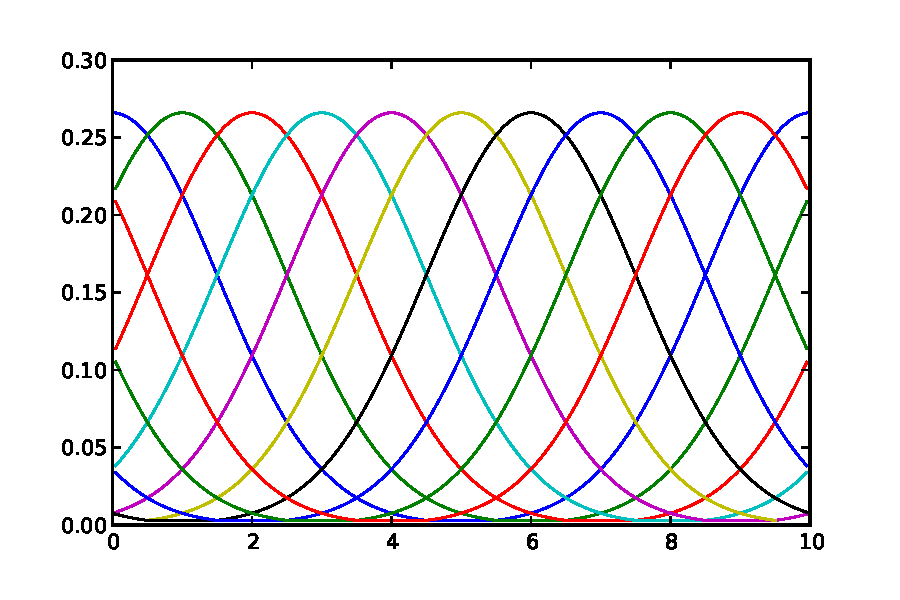
\includegraphics[width=.33\linewidth]{figures/icml-syn1-data.pdf}
  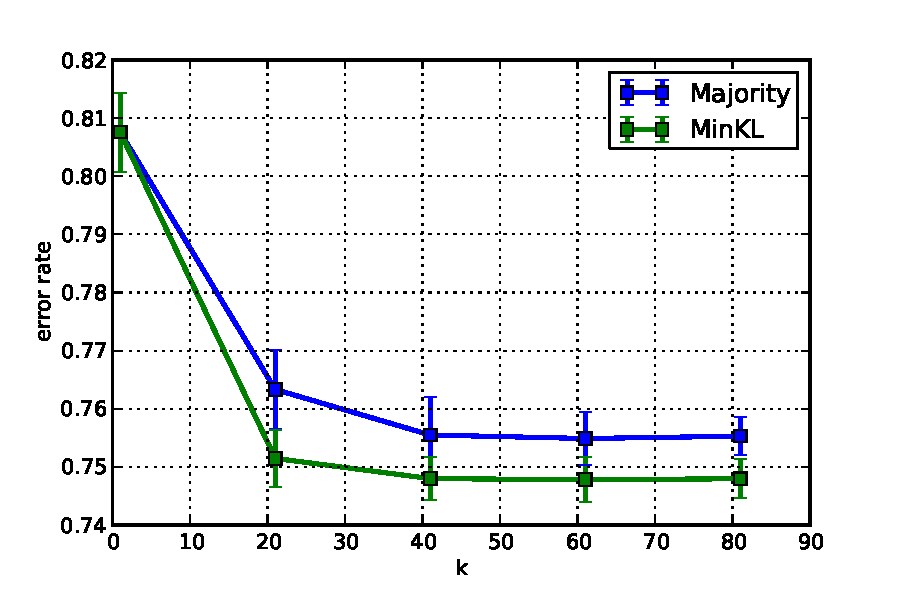
\includegraphics[width=.33\linewidth]{figures/icml-syn1-results-N20.pdf}
  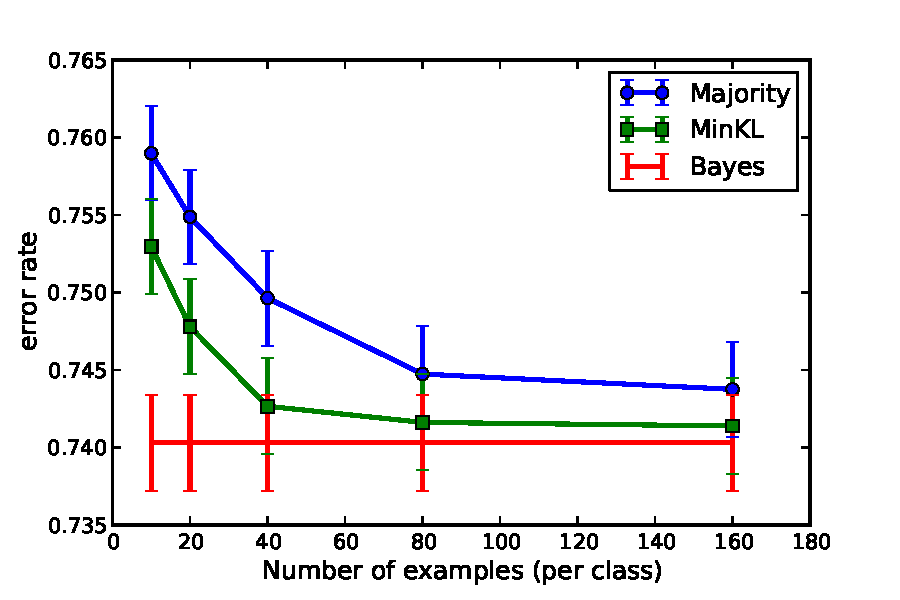
\includegraphics[width=.33\linewidth]{figures/icml-syn1-overall.pdf}
  \label{fig:synthetic-1}
}\\
\subfigure[SYN-2: (left) Data models, (center) error rate vs. $k$
while $n$ fixed, (right) error rate vs. $n$ while $k$ fixed]{
  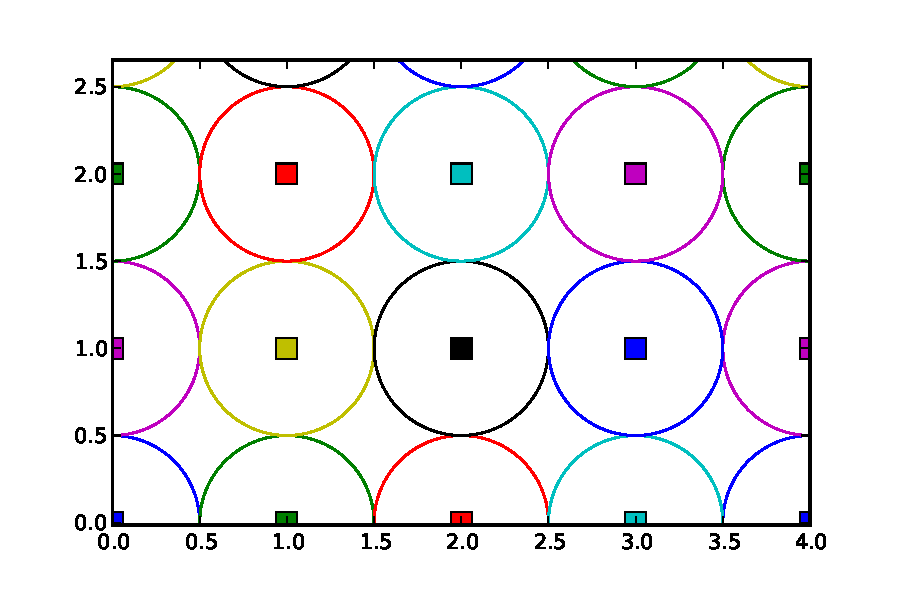
\includegraphics[width=.33\linewidth]{figures/icml-syn2-data.pdf}
  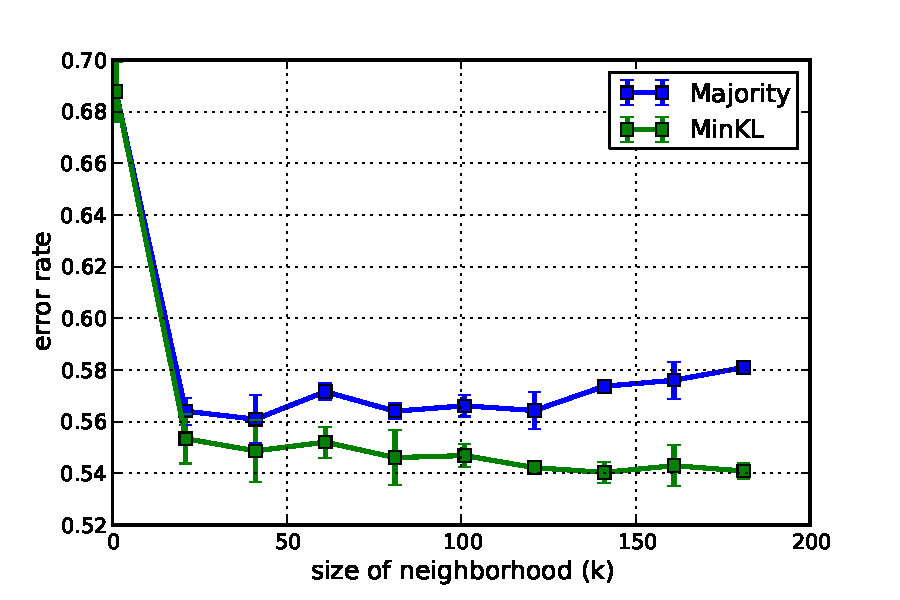
\includegraphics[width=.33\linewidth]{figures/icml-syn2-results-N20.pdf}
  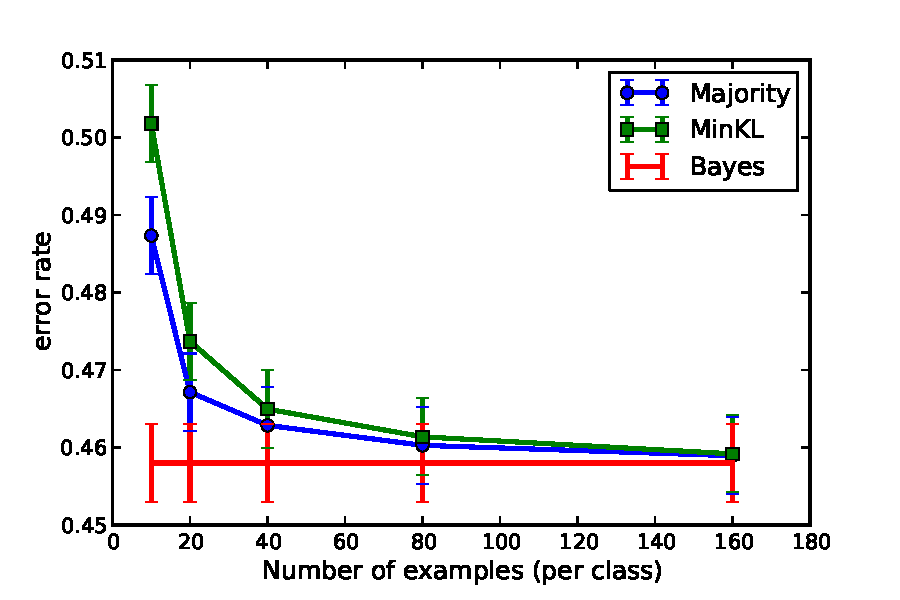
\includegraphics[width=.33\linewidth]{figures/icml-syn3-overall.pdf}
  \label{fig:synthetic-2}
}\\
\subfigure[SYN-3: (left) Data models, (center) error rate vs. $k$
while $n$ fixed, (right) error rate vs. $n$ while $k$ fixed]{
  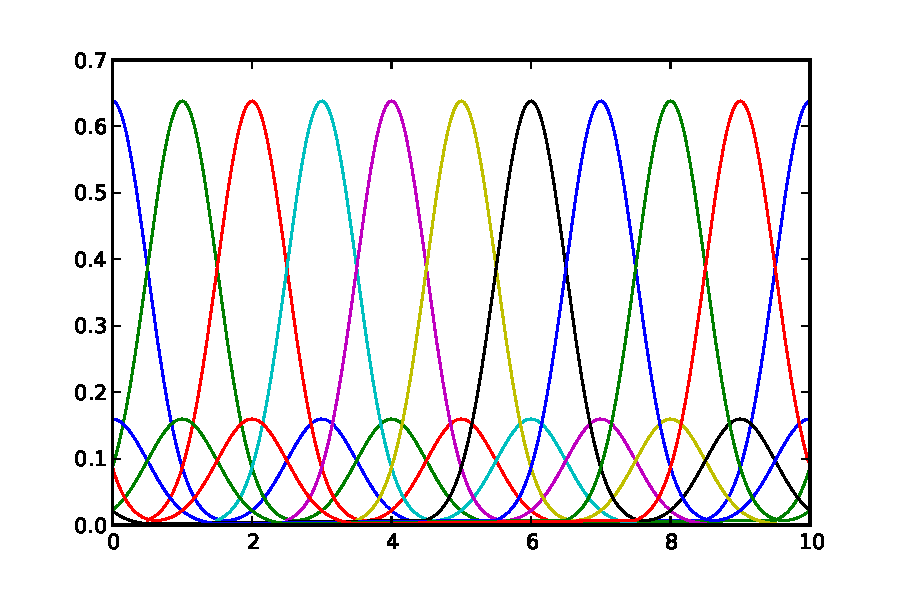
\includegraphics[width=.33\linewidth]{figures/icml-syn3-data.pdf}
  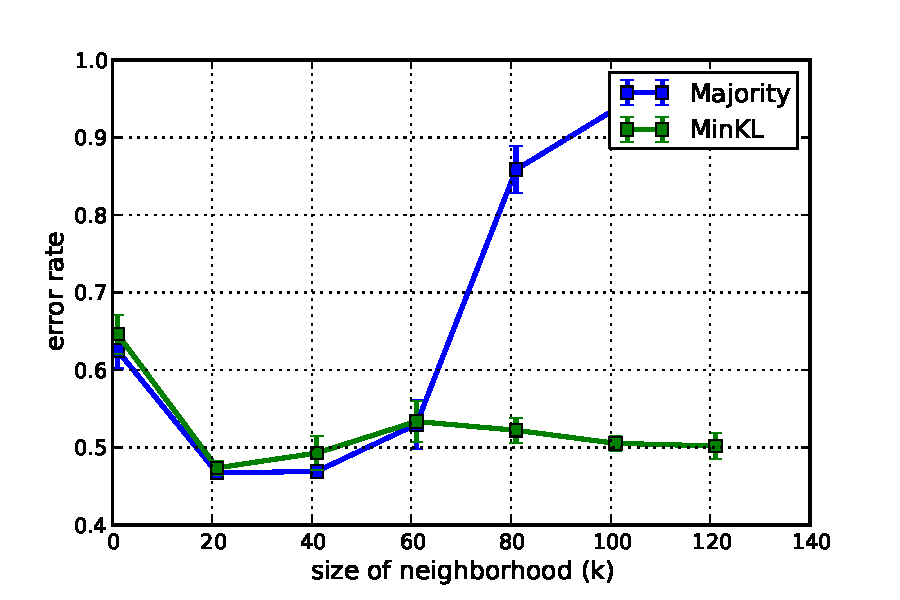
\includegraphics[width=.33\linewidth]{figures/icml-syn3-results-N20.pdf}
  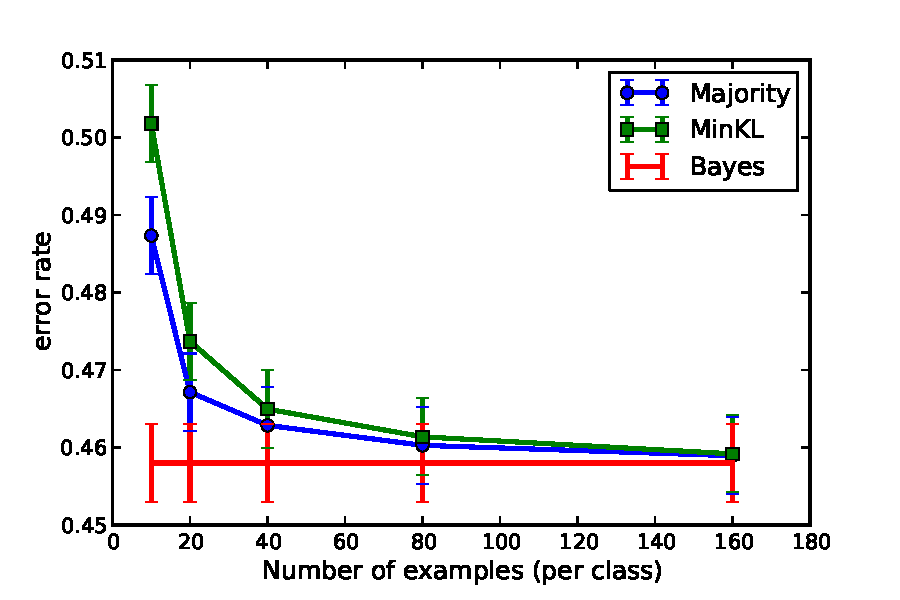
\includegraphics[width=.33\linewidth]{figures/icml-syn3-overall.pdf}
  \label{fig:synthetic-3}
}
\caption{Results from the synthetic data experiment.}
\label{fig:synthetic}
\end{center}
\vskip -0.2in
\end{figure*}

\subsection{uRight}
The uRight dataset contains handwriting trajectories of the 26
lowercase English characters.  We collected the handwriting data from
20 different users writing isolated lowercase English characters on a
touch screen of a mobile phone. Each example is a sequence of
$(x,y,t)$ where $x$ and $y$ are the $(x,y)$-coordinates and $t$ is the
timestamp of each sampling point. Figure~\ref{fig:uright-examples} shows some
examples of the handwriting trajectories. There is a total of 9945
examples and the distribution of the class labels is fairly uniform. The
similarity between two examples is measured by the dynamic time
wraping (DTW) distance~\cite{Bahlmann2004}.

Using $k = 5$, the average error rates of MinKL and Majority for each
user is shown in Figure~\ref{fig:uright-results}. According to the paired
t-test, the average error rate of MinKL (3.76\%) is significantly
smaller than the average error rate of Majority (5.86\%) with $p <
0.001$. The average $\phi$ for the uRight dataset is
0.05. Figure~\ref{fig:uright-mistakes} displays some of the examples that are
misclassified by Majority but not by MinKL.

\begin{figure}[ht]
\vskip 0.2in
\begin{center}
\centering
  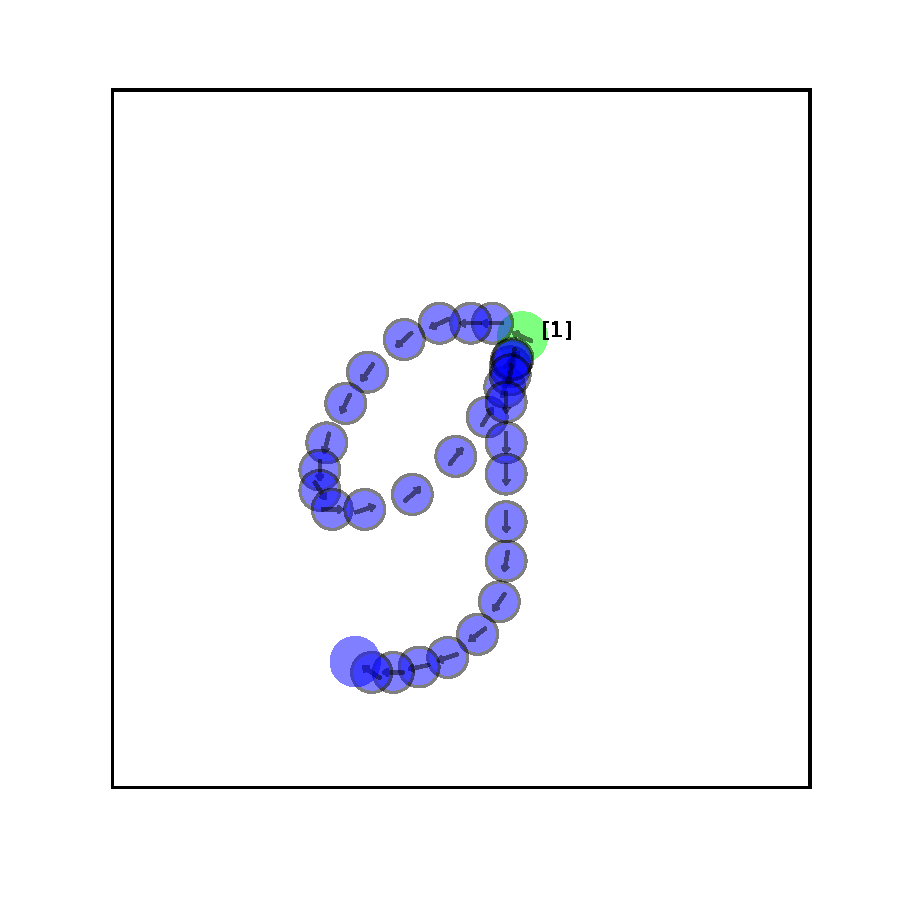
\includegraphics[width=.3\linewidth]{figures/icml-uright-examples-0.pdf}
  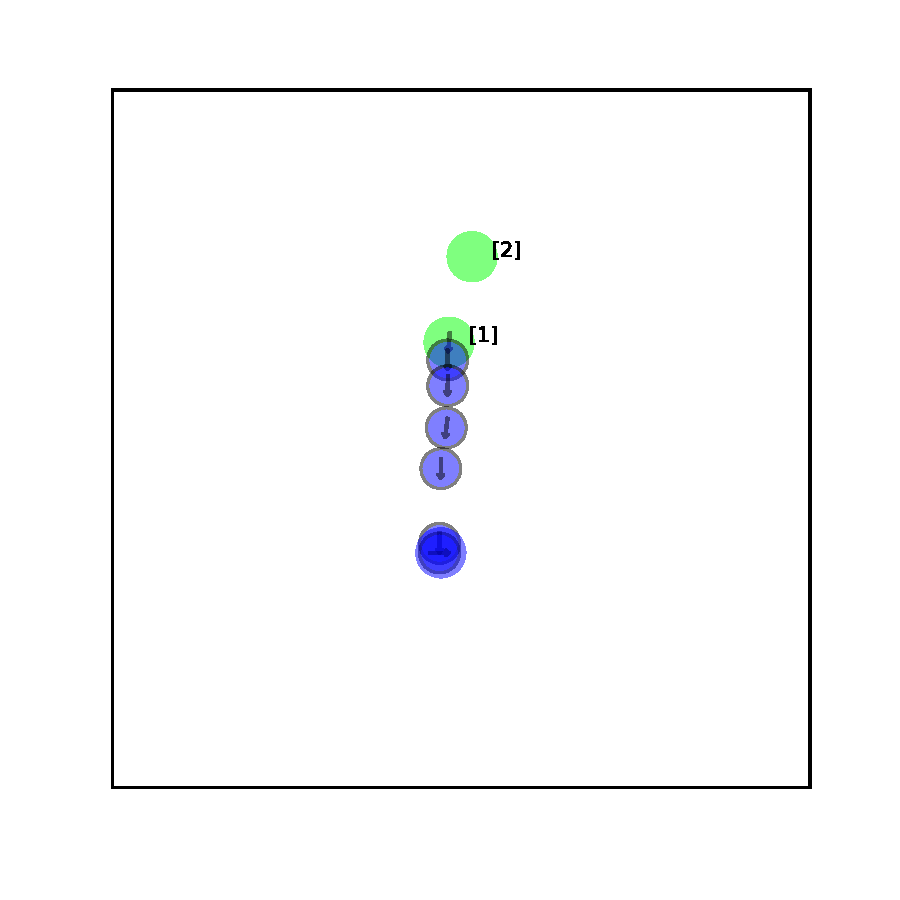
\includegraphics[width=.3\linewidth]{figures/icml-uright-examples-1.pdf}\\
  %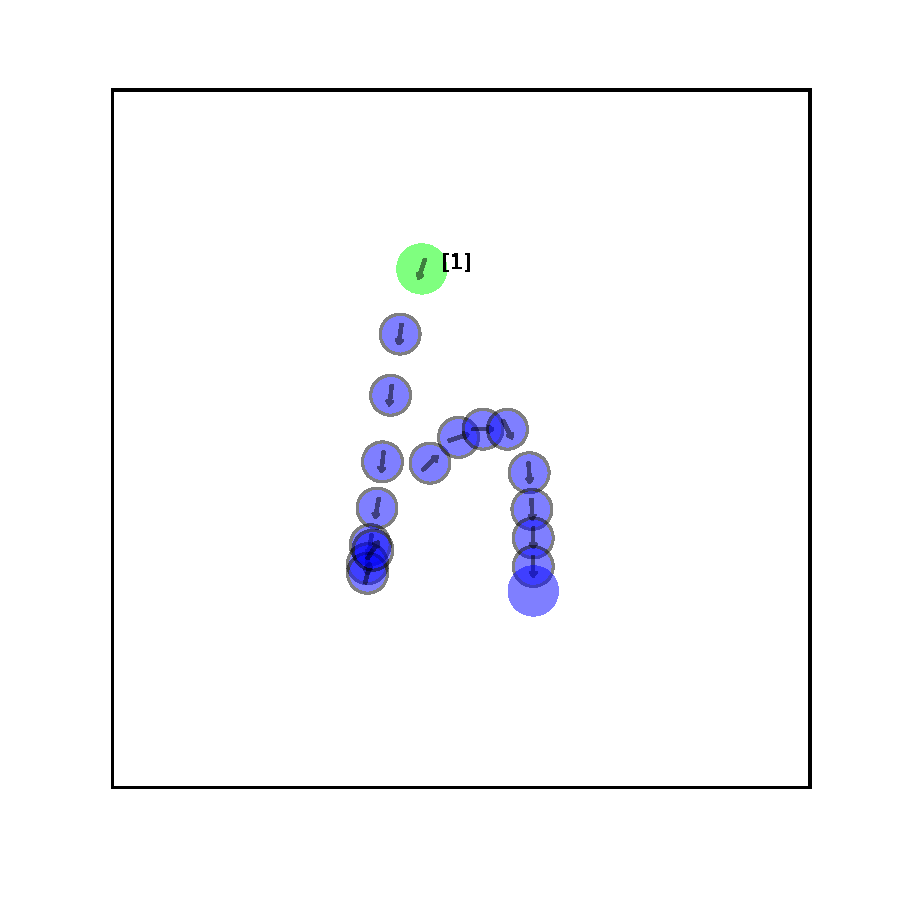
\includegraphics[width=.3\linewidth]{figures/icml-uright-examples-2.pdf}
  %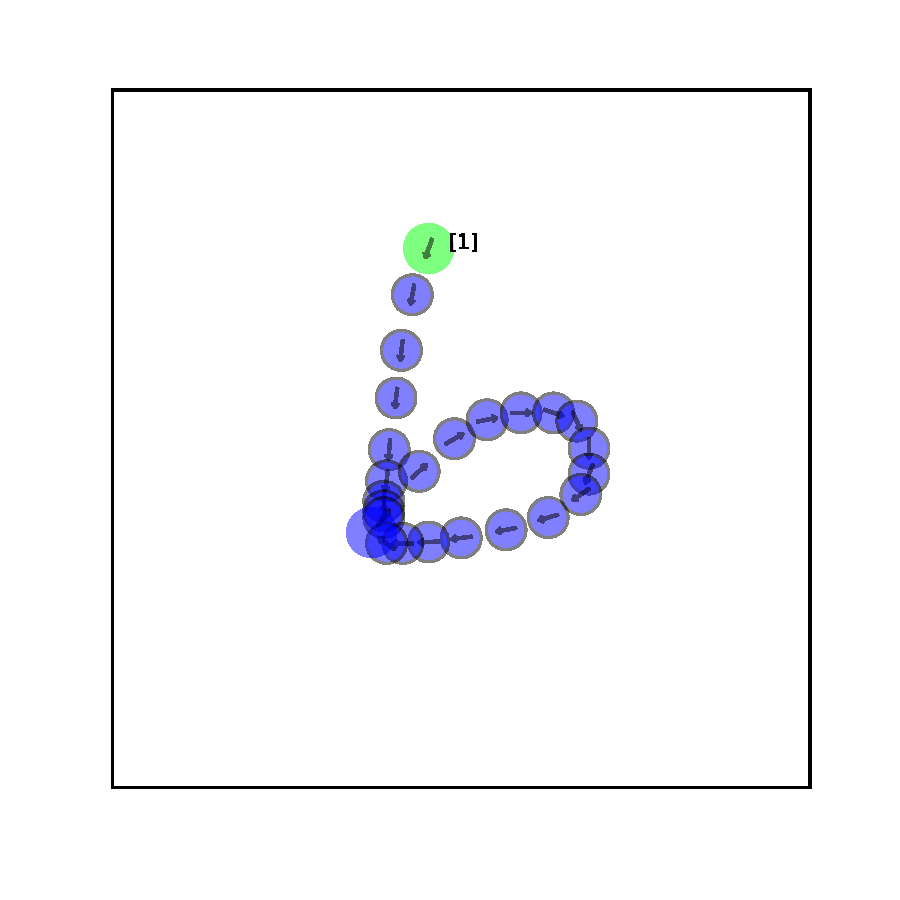
\includegraphics[width=.3\linewidth]{figures/icml-uright-examples-3.pdf}
  \caption{uRight examples}
  \label{fig:uright-examples}
\end{center}
\vskip -0.2in
\end{figure}

\begin{figure}[ht]
\vskip 0.2in
\begin{center}
\centering
  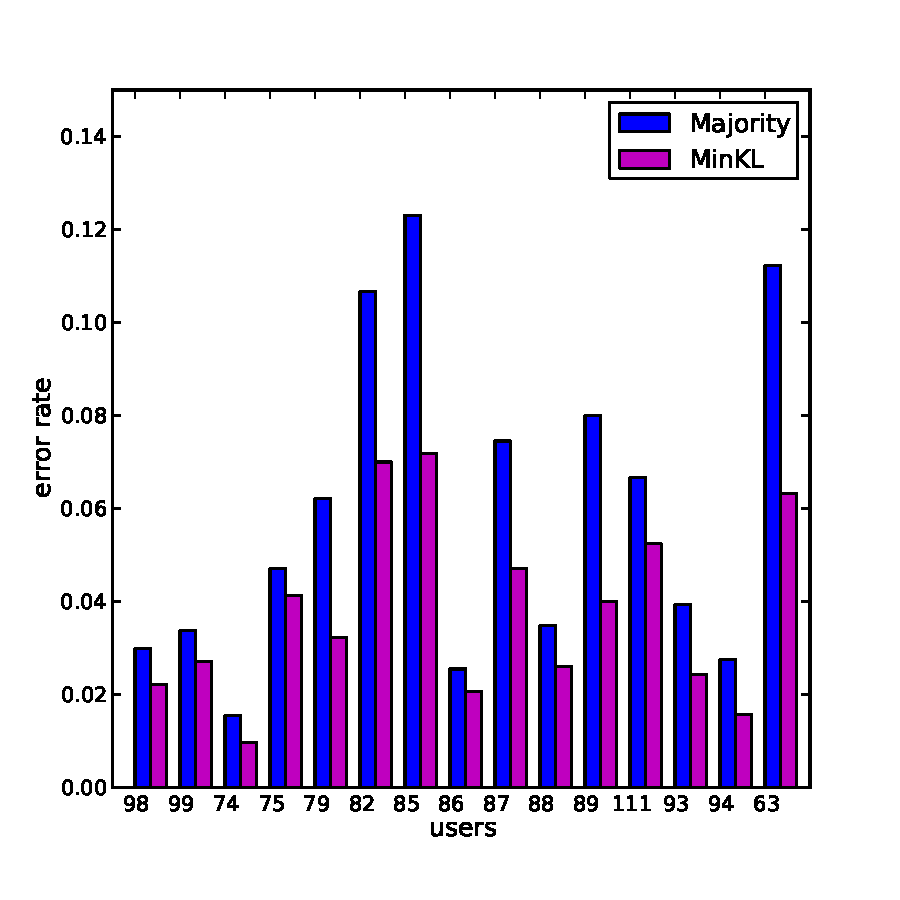
\includegraphics[width=.95\linewidth]{figures/icml-uright-allusers.pdf}
  \caption{uRight results}
  \label{fig:uright-results}
\end{center}
\vskip -0.2in
\end{figure}

\begin{figure}[ht]
\vskip 0.2in
\begin{center}
\centering
  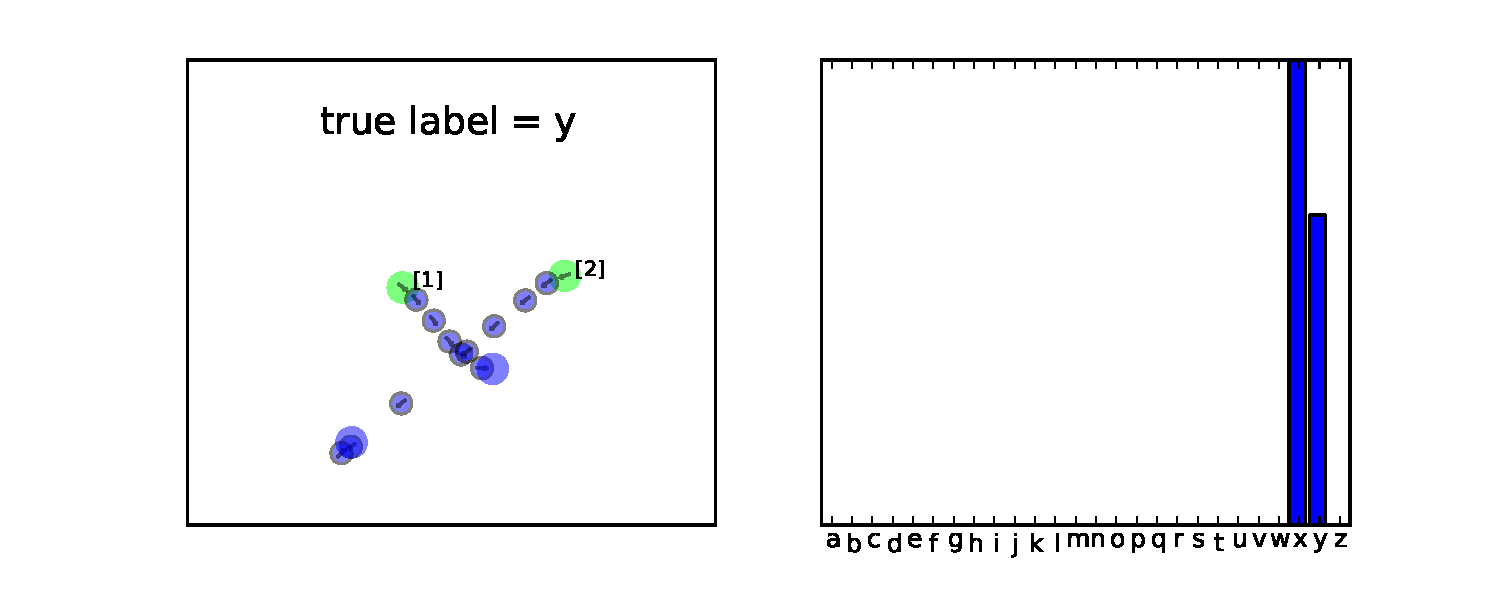
\includegraphics[width=.95\linewidth]{figures/icml-uright-interesting-134.pdf}\\
  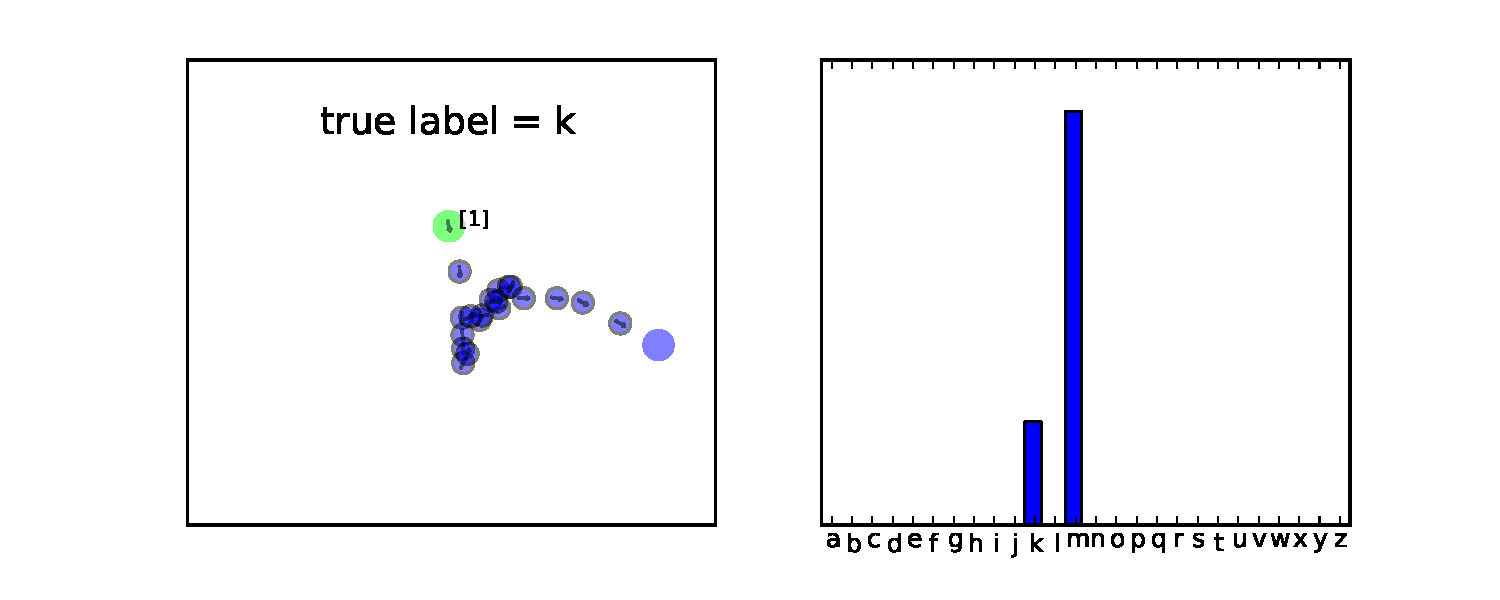
\includegraphics[width=.95\linewidth]{figures/icml-uright-interesting-70.pdf}\\
  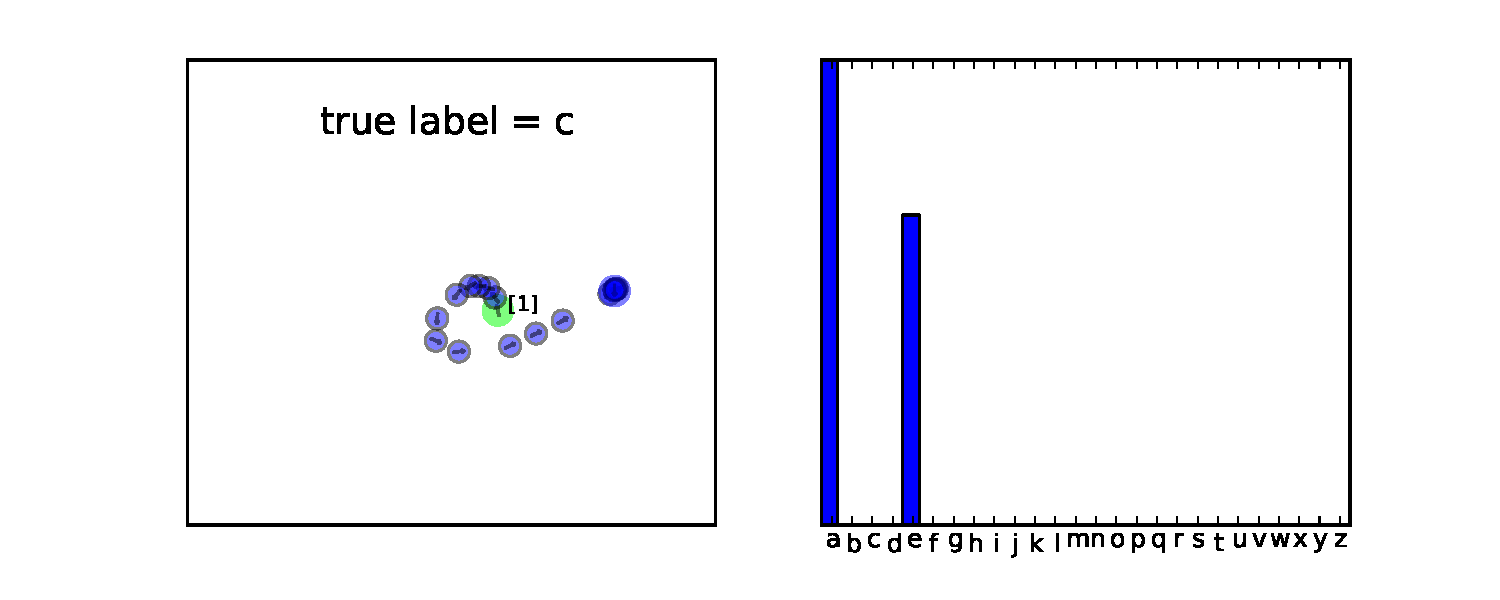
\includegraphics[width=.95\linewidth]{figures/icml-uright-interesting-248.pdf}\\
  \caption{uRight mistakes}
  \label{fig:uright-mistakes}
\end{center}
\vskip -0.2in
\end{figure}

\begin{figure}[ht]
\vskip 0.2in
\begin{center}
\centering
  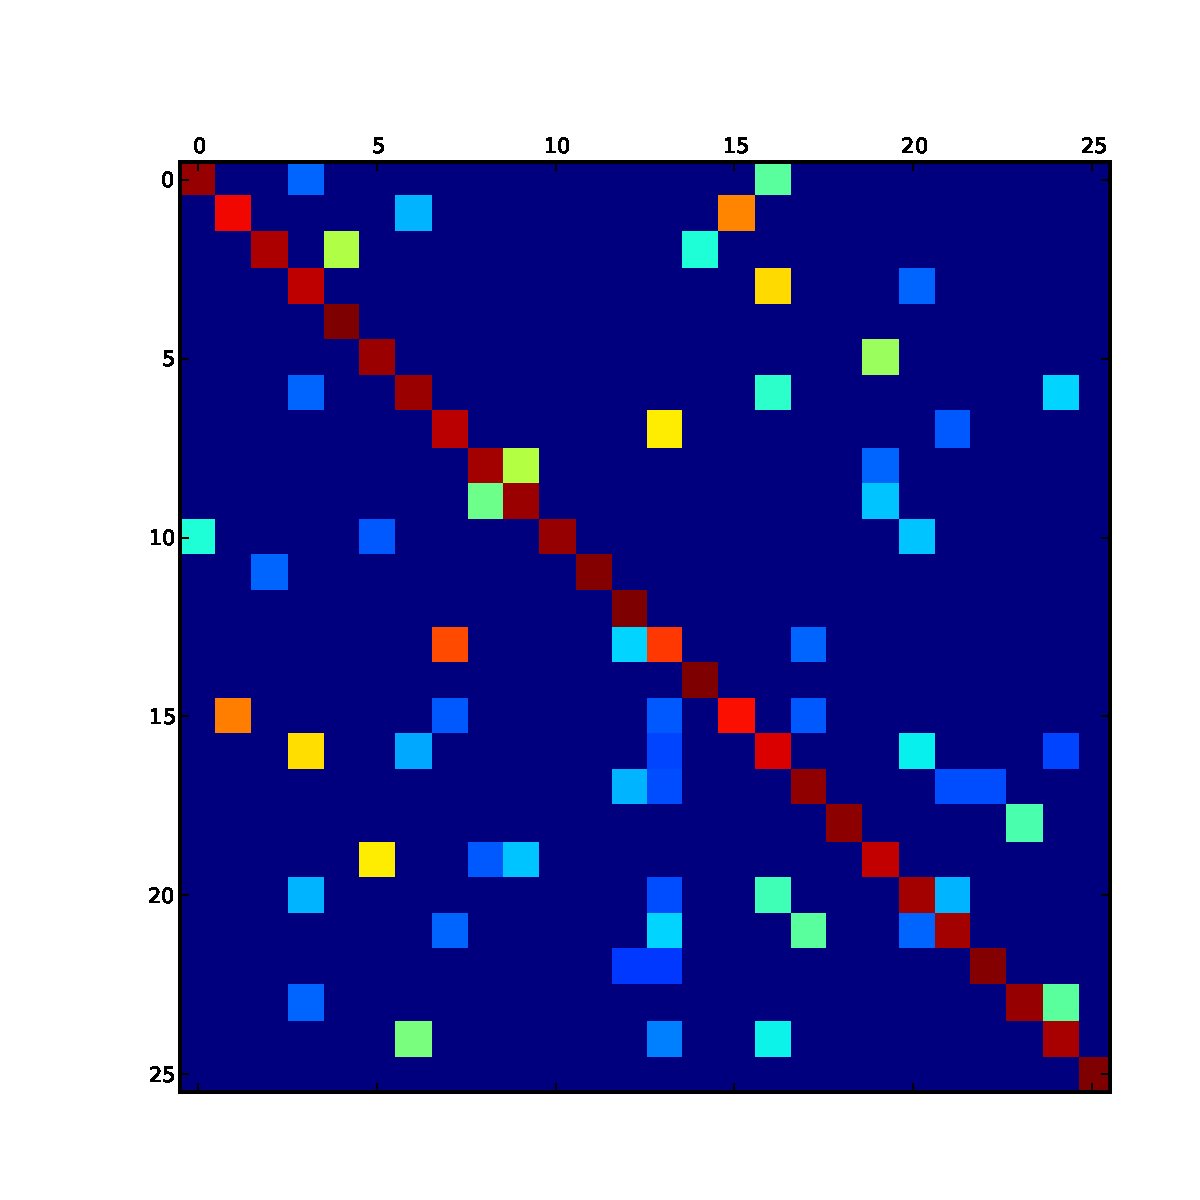
\includegraphics[width=.95\linewidth]{figures/icml-uright-matrix-82.pdf}\\
  \caption{uRight matrix}
  \label{fig:uright-matrix}
\end{center}
\vskip -0.2in
\end{figure}


\subsection{MNIST}
The MNIST dataset~\cite{Lecun1998} contains images of digits. Each
example is a 28x28 grayscale image and there are a total of 60000
training examples and 10000 test examples in the dataset. We
prepropress the data by deskewing, downsampling the images. The
feature vector of each example corresponds to the top 100 PCA
components of the preprocessed image. The Euclidean distance is used
as the similarity measure in the neighborhood calculation.

Figure~\ref{fig:mnist} shows the test error rates
of the two algorithm obtained at different $k$.The $\phi$ of MNIST
dataset is 0.05.

\begin{figure}[ht]
\vskip 0.2in
\begin{center}
\centering
  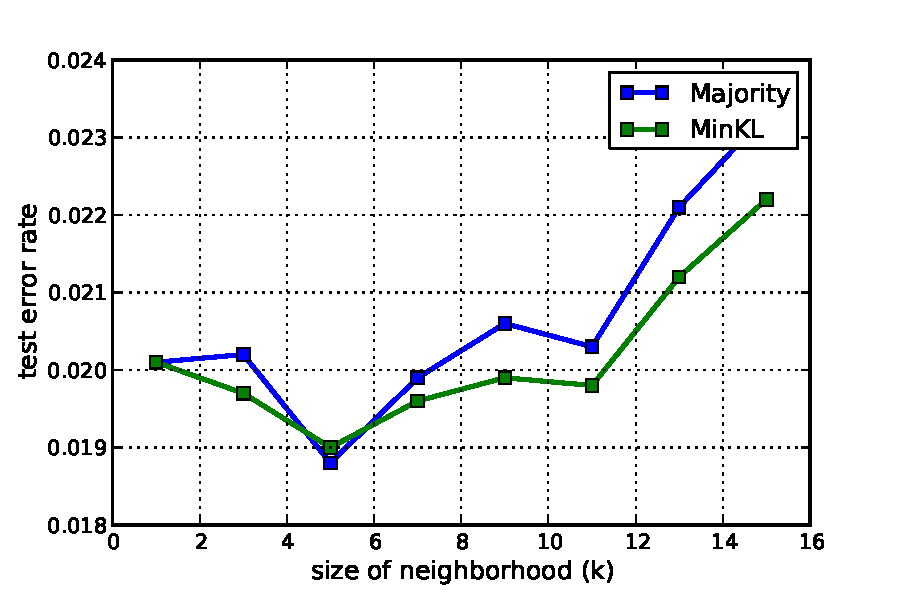
\includegraphics[width=.95\linewidth]{figures/icml-mnist-error.pdf}
  \caption{MNIST results}
  \label{fig:mnist-results}
\end{center}
\vskip -0.2in
\end{figure}


\subsection{SVHN}
The SVHN dataset~\cite{Netzer2011} contains images of digits taken
from the Google street view data. It is considered a harder dataset
than MNIST. Each example in SVHN is a 32x32 RGB image patch and there
are a total of 73257 training examples and 26032 test examples in the
dataset. For each example, HOG features~\cite{Dalal2005} are computed
and combined into a feature vector. We use 4x4 The Manhattan distance is used as
the similarity measure in the neighborhood calculation.

The results are summarized in Figure~\ref{}.

\begin{figure}[ht]
\vskip 0.2in
\begin{center}
\centering
  \includegraphics[width=.95\linewidth]{figures/svhn-1.png}
  \caption{SVHN results}
  \label{fig:svhn-results}
\end{center}
\vskip -0.2in
\end{figure}

\section{Discussion}

From the \textbf{SYN-1} and \textbf{SYN-2} experiments, we observe
that MinKL performs significantly better than Majority, especially
when $n$ is small. As the number of training examples increases, the
performance gap of the two approaches decreases. This is not
surprising because the majority vote rule is known to be optimal
asymptotically. However, in some applications where the number of
training examples is limited, our approach has advantage over the
majority rule.

MNIST and SVHN have small $\phi$ but the noise is small and evenly distributed.


As we expected, the MinKL approach performs well when $\phi$ is
small. This gives us a simple way to check if a problem is suitable
for MinKL. 


We suspect that our approach will be more beneficial to problems with
a large number of classes and the confusions between classes are
non-uniform.


In a sense, our approach naturally incoporates the infomation from the
label space into the classification. The label space information is
encoded into the prototypical neighborhood distribution. The
performance of our approach depends on how different the prototypical
neighborhood distributions of different classes are. If the
prototypical distributions are similar to each other, then our
approach will not perform well. A workaround is to maintain multiple
prototypical distributions per class.

Our approach does not have a consistency gaurantee. It is
possible that our approach will be sub-optimal when the number of
training examples goes to infinity because the prototypical
distribution model is incorrect or insufficent. We do not worry
about this problem that much since we see our approach being used
in a small sample scenario.

In practice, other divergences might work better than the
KL-divergence. The KL-divergence is considered a special case of a
more general divergence function called
Alpha-divergence~\cite{Cichocki2010}, which is given by
\[
D^{(\alpha)}_A (p||q) = \frac{1}{\alpha(\alpha - 1)}\left( \sum_1^n
  p^{\alpha}_i q^{1-\alpha}_i - 1\right), \; \alpha \in \mathrm{R} \ \{0,1\}
\]
The KL-divergence can be expressed as $D_{KL} (p || q) = \lim_{\alpha
  \rightarrow 1} D^{(\alpha)}_A (p || q)$.  For the uRight dataset, we
were able to obtain even lower error rate by using Alpha-divergence
with $\alpha = 2$.

Our approach can be applied to other classification algorithms as
well. The $k$-NN algorithm is very computational expensive in
classifying a new example. In some applications, it is important to be
able to classify new examples quickly. A simple modification to the
$k$-NN algorithm that significanly reduces the classication time is to
keep only a small number of representatives per class and discard the
rest of the examples. This algorithm is called the $k$
nearest-centroid algorithm ($k$-NC) where only the $k$-centroids are
kept as the class representatives. In the $k$-NC, the class
distribution $\mathbf{P}_x$ can be estimating by
\[
\mathbf{P}_x(j) = \frac{e^{d(x,C(j))}}{\sum_i e^{d(x, C(i))} }
\]
We can apply MinKL to the class posterior computed this
way. In Figure~\ref{}, we compare the accuracy of the $k$-NC algorithm
with MinKL and Maximum (equavalent to Majority in the $k$-NN).

\section{Conclusions}

We suggest a simple modification to the $k$-NN algorithm.

\bibliography{library}
\bibliographystyle{icml2014}

\end{document} 


% This document was modified from the file originally made available by
% Pat Langley and Andrea Danyluk for ICML-2K. This version was
% created by Lise Getoor and Tobias Scheffer, it was slightly modified  
% from the 2010 version by Thorsten Joachims & Johannes Fuernkranz, 
% slightly modified from the 2009 version by Kiri Wagstaff and 
% Sam Roweis's 2008 version, which is slightly modified from 
% Prasad Tadepalli's 2007 version which is a lightly 
% changed version of the previous year's version by Andrew Moore, 
% which was in turn edited from those of Kristian Kersting and 
% Codrina Lauth. Alex Smola contributed to the algorithmic style files.  
